
\documentclass[a4paper,12pt,twoside]{report}
\usepackage[left=2cm,right=2cm,top=2cm,bottom=3cm]{geometry}
\usepackage[inline]{enumitem}
\usepackage[utf8]{inputenc}
\usepackage{hyperref}
\usepackage{natbib}
\usepackage{authordate1-4}
\usepackage{appendix}
\usepackage[nottoc]{tocbibind} % add Bibliography to toc
\usepackage{caption}
\usepackage{subcaption}
\usepackage{booktabs}
\usepackage{longtable}
\usepackage{algorithm2e}
\usepackage{float}
\restylefloat{table}

\hypersetup{linktoc=all}
% \usepackage{url}


\usepackage{graphicx}
\usepackage{verbatim}
\usepackage{latexsym}
\usepackage{mathchars}
\usepackage{setspace}

\setlength{\parskip}{\medskipamount}  % a little space before a \par
\setlength{\parindent}{0pt}	      % don't indent first lines of paragraphs

%UHEAD.STY  If this is included after \documentstyle{report}, it adds
% an underlined heading style to the LaTeX report style.
% \pagestyle{uheadings} will put underlined headings at the top
% of each page. The right page headings are the Chapter titles and
% the left page titles are supplied by \def\lefthead{text}.

% Ted Shapin, Dec. 17, 1986

\makeatletter
\def\chapapp2{Chapter}

\def\appendix{\par
 \setcounter{chapter}{0}
 \setcounter{section}{0}
 \def\chapapp2{Appendix}
 \def\@chapapp{Appendix}
 \def\thechapter{\Alph{chapter}}}

\def\ps@uheadings{\let\@mkboth\markboth
% modifications
\def\@oddhead{\protect\underline{\protect\makebox[\textwidth][l]
		{\sl\rightmark\hfill\rm\thepage}}}
\def\@oddfoot{}
\def\@evenfoot{}
\def\@evenhead{\protect\underline{\protect\makebox[\textwidth][l]
		{\rm\thepage\hfill\sl\leftmark}}}
% end of modifications
\def\chaptermark##1{\markboth {\ifnum \c@secnumdepth >\m@ne
 \chapapp2\ \thechapter. \ \fi ##1}{}}%
\def\sectionmark##1{\markright {\ifnum \c@secnumdepth >\z@
   \thesection. \ \fi ##1}}}
\makeatother



%%From: marcel@cs.caltech.edu (Marcel van der Goot)
%%Newsgroups: comp.text.tex
%%Subject: illegal modification of boxit.sty
%%Date: 28 Feb 92 01:10:02 GMT
%%Organization: California Institute of Technology (CS dept)
%%Nntp-Posting-Host: andromeda.cs.caltech.edu
%%
%%
%%Quite some time ago I posted a file boxit.sty; maybe it made it
%%to some archives, although I don't recall submitting it. It defines
%%	\begin{boxit}
%%	...
%%	\end{boxit}
%%to draw a box around `...', where the `...' can contain other
%%environments (e.g., a verbatim environment). Unfortunately, it had
%%a problem: it did not work if you used it in paragraph mode, i.e., it
%%only worked if there was an empty line in front of \begin{boxit}.
%%Luckily, that is easily corrected.
%%
%%HOWEVER, apparently someone noticed the problem, tried to correct it,
%%and then distributed this modified version. That would be fine with me,
%%except that:
%%1. There was no note in the file about this modification, it only has my
%%   name in it.
%%2. The modification is wrong: now it only works if there is *no* empty
%%   line in front of \begin{boxit}. In my opinion this bug is worse than
%%   the original one.
%%
%%In particular, the author of this modification tried to force an empty
%%line by inserting a `\\' in the definition of \Beginboxit. If you have
%%a version of boxit.sty with a `\\', please delete it. If you have my
%%old version of boxit.sty, please also delete it. Below is an improved
%%version.
%%
%%Thanks to Joe Armstrong for drawing my attention to the bug and to the
%%illegal version.
%%
%%                                          Marcel van der Goot
%% .---------------------------------------------------------------
%% | Blauw de viooltjes,                    marcel@cs.caltech.edu
%% |    Rood zijn de rozen;
%% | Een rijm kan gezet
%% |    Met plaksel en dozen.
%% |


% boxit.sty
% version: 27 Feb 1992
%
% Defines a boxit environment, which draws lines around its contents.
% Usage:
%   \begin{boxit}
%	... (text you want to be boxed, can contain other environments)
%   \end{boxit}
%
% The width of the box is the width of the contents.
% The boxit* environment behaves the same, except that the box will be
% at least as wide as a normal paragraph.
%
% The reason for writing it this way (rather than with the \boxit#1 macro
% from the TeXbook), is that now you can box verbatim text, as in
%   \begin{boxit}
%   \begin{verbatim}
%   this better come out in boxed verbatim mode ...
%   \end{verbatim}
%   \end{boxit}
%
%						Marcel van der Goot
%						marcel@cs.caltech.edu
%

\def\Beginboxit
   {\par
    \vbox\bgroup
	   \hrule
	   \hbox\bgroup
		  \vrule \kern1.2pt %
		  \vbox\bgroup\kern1.2pt
   }

\def\Endboxit{%
			      \kern1.2pt
		       \egroup
		  \kern1.2pt\vrule
		\egroup
	   \hrule
	 \egroup
   }	

\newenvironment{boxit}{\Beginboxit}{\Endboxit}
\newenvironment{boxit*}{\Beginboxit\hbox to\hsize{}}{\Endboxit}

\pagestyle{empty}

\setlength{\parskip}{2ex plus 0.5ex minus 0.2ex}
\setlength{\parindent}{0pt}

\makeatletter  %to avoid error messages generated by "\@". Makes Latex treat "@" like a letter

\linespread{0.66}
\def\submitdate#1{\gdef\@submitdate{#1}}

\def\maketitle{
  \begin{titlepage}{
    %\linespread{1.5}
    \Large Queen Mary, University of London \\
    %\linebreak
    Department of Electronic Engineering and Computer Science
    \rm
    \vskip 3in
    \Large \bf \@title \par
  }
  \vskip 0.3in
  \par
  {\Large \@author}
  \vskip 0.1in
  {\Large Supervisor: Dr. Matthew Purver}

  \vskip 4in
  \par
  Submitted in part fulfilment of the requirements for the degree of
  \linebreak
  BSc Computer Science with Industrial Experience, \@submitdate
  \vfil
  \end{titlepage}
}

\def\titlepage{
  \newpage
  \centering
  \linespread{1}
  \normalsize
  \vbox to \vsize\bgroup\vbox to 9in\bgroup
}
\def\endtitlepage{
  \par
  \kern 0pt
  \egroup
  \vss
  \egroup
  \cleardoublepage
}

\def\abstract{
  \begin{center}{
    \large\bf Abstract}
  \end{center}
  \small
  %\def\baselinestretch{1.5}
  \linespread{1.5}
  \normalsize
}
\def\endabstract{
  \par
}

\newenvironment{acknowledgements}{
  \cleardoublepage
  \begin{center}{
    \large \bf Acknowledgements}
  \end{center}
  \small
  \linespread{1.5}
  \normalsize
}{\cleardoublepage}
\def\endacknowledgements{
  \par
}

\newenvironment{dedication}{
  \cleardoublepage
  \begin{center}{
    \large \bf Dedication}
  \end{center}
  \small
  \linespread{1.5}
  \normalsize
}{\cleardoublepage}
\def\enddedication{
  \par
}

\def\preface{
    \pagenumbering{roman}
    \pagestyle{plain}
    \doublespacing
}

\def\body{
    \cleardoublepage
    \pagestyle{uheadings}
    \tableofcontents
    \pagestyle{plain}

    \cleardoublepage
    \pagestyle{uheadings}
    \listoftables
    \pagestyle{plain}

    \cleardoublepage
    \pagestyle{uheadings}
    \listoffigures
    \pagestyle{plain}

    \cleardoublepage
    \pagestyle{uheadings}
    \pagenumbering{arabic}
    % \doublespacing
}

\makeatother  %to avoid error messages generated by "\@". Makes Latex treat "@" like a letter


\newcommand{\ipc}{{\sf ipc}}

\newcommand{\Prob}{\bbbp}
\newcommand{\Real}{\bbbr}
\newcommand{\real}{\Real}
\newcommand{\Int}{\bbbz}
\newcommand{\Nat}{\bbbn}

\newcommand{\NN}{{\sf I\kern-0.14emN}}   % Natural numbers
\newcommand{\ZZ}{{\sf Z\kern-0.45emZ}}   % Integers
\newcommand{\QQQ}{{\sf C\kern-0.48emQ}}   % Rational numbers
\newcommand{\RR}{{\sf I\kern-0.14emR}}   % Real numbers
\newcommand{\KK}{{\cal K}}
\newcommand{\OO}{{\cal O}}
\newcommand{\AAA}{{\bf A}}
\newcommand{\HH}{{\bf H}}
\newcommand{\II}{{\bf I}}
\newcommand{\LL}{{\bf L}}
\newcommand{\PP}{{\bf P}}
\newcommand{\PPprime}{{\bf P'}}
\newcommand{\QQ}{{\bf Q}}
\newcommand{\UU}{{\bf U}}
\newcommand{\UUprime}{{\bf U'}}
\newcommand{\zzero}{{\bf 0}}
\newcommand{\ppi}{\mbox{\boldmath $\pi$}}
\newcommand{\aalph}{\mbox{\boldmath $\alpha$}}
\newcommand{\bb}{{\bf b}}
\newcommand{\ee}{{\bf e}}
\newcommand{\mmu}{\mbox{\boldmath $\mu$}}
\newcommand{\vv}{{\bf v}}
\newcommand{\xx}{{\bf x}}
\newcommand{\yy}{{\bf y}}
\newcommand{\zz}{{\bf z}}
\newcommand{\oomeg}{\mbox{\boldmath $\omega$}}
\newcommand{\res}{{\bf res}}
\newcommand{\cchi}{{\mbox{\raisebox{.4ex}{$\chi$}}}}
%\newcommand{\cchi}{{\cal X}}
%\newcommand{\cchi}{\mbox{\Large $\chi$}}

% Logical operators and symbols
\newcommand{\imply}{\Rightarrow}
\newcommand{\bimply}{\Leftrightarrow}
\newcommand{\union}{\cup}
\newcommand{\intersect}{\cap}
\newcommand{\boolor}{\vee}
\newcommand{\booland}{\wedge}
\newcommand{\boolimply}{\imply}
\newcommand{\boolbimply}{\bimply}
\newcommand{\boolnot}{\neg}
\newcommand{\boolsat}{\!\models}
\newcommand{\boolnsat}{\!\not\models}


\newcommand{\op}[1]{\mathrm{#1}}
\newcommand{\s}[1]{\ensuremath{\mathcal #1}}

% Properly styled differentiation and integration operators
\newcommand{\diff}[1]{\mathrm{\frac{d}{d\mathit{#1}}}}
\newcommand{\diffII}[1]{\mathrm{\frac{d^2}{d\mathit{#1}^2}}}
\newcommand{\intg}[4]{\int_{#3}^{#4} #1 \, \mathrm{d}#2}
\newcommand{\intgd}[4]{\int\!\!\!\!\int_{#4} #1 \, \mathrm{d}#2 \, \mathrm{d}#3}

% Large () brackets on different lines of an eqnarray environment
\newcommand{\Leftbrace}[1]{\left(\raisebox{0mm}[#1][#1]{}\right.}
\newcommand{\Rightbrace}[1]{\left.\raisebox{0mm}[#1][#1]{}\right)}

% Funky symobols for footnotes
\newcommand{\symbolfootnote}{\renewcommand{\thefootnote}{\fnsymbol{footnote}}}
% now add \symbolfootnote to the beginning of the document...

\newcommand{\normallinespacing}{\renewcommand{\baselinestretch}{1.5} \normalsize}
\newcommand{\mediumlinespacing}{\renewcommand{\baselinestretch}{1.2} \normalsize}
\newcommand{\narrowlinespacing}{\renewcommand{\baselinestretch}{1.0} \normalsize}
\newcommand{\bump}{\noalign{\vspace*{\doublerulesep}}}
\newcommand{\cell}{\multicolumn{1}{}{}}
\newcommand{\spann}{\mbox{span}}
\newcommand{\diagg}{\mbox{diag}}
\newcommand{\modd}{\mbox{mod}}
\newcommand{\minn}{\mbox{min}}
\newcommand{\andd}{\mbox{and}}
\newcommand{\forr}{\mbox{for}}
\newcommand{\EE}{\mbox{E}}

\newcommand{\deff}{\stackrel{\mathrm{def}}{=}}
\newcommand{\syncc}{~\stackrel{\textstyle \rhd\kern-0.57em\lhd}{\scriptstyle L}~}

\def\coop{\mbox{\large $\rhd\!\!\!\lhd$}}
\newcommand{\sync}[1]{\raisebox{-1.0ex}{$\;\stackrel{\coop}{\scriptscriptstyle
#1}\,$}}

\newtheorem{definition}{Definition}[chapter]
\newtheorem{theorem}{Theorem}[chapter]

\newcommand{\Sectionref}[1]{Section~\ref{#1}}
\newcommand{\Tableref}[1]{Table~\ref{#1}}
\newcommand{\Pageref}[1]{page~\pageref{#1}}

\newcommand{\Figref}[1]{Figure~\ref{#1}}
\newcommand{\fig}[3]{
 \begin{figure}[!ht]
 \begin{center}
 \scalebox{#3}{\includegraphics{figs/#1.ps}}
 \vspace{-0.1in}
 \caption[ ]{\label{#1} #2}
 \end{center}
 \end{figure}
}

\newcommand{\figtwo}[8]{
 \begin{figure}
 \parbox[b]{#4 \textwidth}{
 \begin{center}
 \scalebox{#3}{\includegraphics{figs/#1.ps}}
 \vspace{-0.1in}
 \caption{\label{#1}#2}
 \end{center}
 }
 \hfill
 \parbox[b]{#8 \textwidth}{
 \begin{center}
 \scalebox{#7}{\includegraphics{figs/#5.ps}}
 \vspace{-0.1in}
 \caption{\label{#5}#6}
 \end{center}
 }
 \end{figure}
}

\setcounter{secnumdepth}{4}
\setcounter{tocdepth}{4}

\begin{document}

\title{\LARGE {\bf Discovering Themes in Social Media}\\
 \vspace*{6mm}
}

\author{Fayimora Femi-Balogun}
\supervisor{Dr. Matthew Purver}
\submitdate{April 2014}
\normallinespacing
\maketitle

\preface

\addcontentsline{toc}{chapter}{Abstract}

\begin{abstract}

Text of the Abstract.

\end{abstract}


\cleardoublepage

\addcontentsline{toc}{chapter}{Acknowledgements}

\begin{acknowledgements}

% I would like to express (whatever feelings I have) to:
%
% \begin{itemize}
%  \item My supervisor
%  \vspace*{3mm}
%  \item Other researchers
%  \vspace*{3mm}
%  \item My family and friends
% \end{itemize}
%
\end{acknowledgements}


\cleardoublepage

\begin{dedication}
  Dedication here.
\end{dedication}


\clearpage

\null\vfill\vfill % Add some space to move the quote down the page a bit


\textit{``No amount of experimentation can ever prove me right; a single experiment can prove me
wrong.''}

\begin{flushright}
Albert Einstein
\end{flushright}

\vfill\vfill\vfill\vfill\vfill\vfill\null % Add some space at the bottom to position the quote just right



\body

\chapter{Introduction}
% In this chapter, we discuss the aims and objectives of this study.


\section{Motivation and Objectives}
The main aim of this project is to investigate the use of Machine Learning and Natural Language
Processing techniques on social data. Every organisation today is continuously search for new ways
to get feedback from their clients/users. Current ways of achieving this include
\textbf{Surveys} (questionaires or interviews) and \textbf{Focus Groups}.

Surveys have the advantage being very easy to create. There are also a variety of tools to help with
this. Some of them include SurveyMonkey\footnote{https://www.surveymonkey.com/}, Google
Docs\footnote{https://drive.google.com}. Unfortunately, Surveys also have a few unpleasant drawbacks
like time consumption and labour intensity. It can also be difficult to encourage partcipants to
respond. Nonetheless, the main drawback to using Surveys is that the some questions are left
unanswered while the answers given may not reflect the truthful sentiments of the
participant.~\cite{DonaldBRubin1987} concurs with this and he goes on to discuss how this problem
can be solved (to a certain extent) with imputation\footnote{Imputation is the process of inferring
plausible values for missing entries}.~\cite{BobEHayes2008} also agrees with this point of view and
suggests the use of well designed leading questions to put the participant in the right frame of
mind. For instance, a leading question like ``\textit{How likely will you recommend our service to
friends?}'' gets the participant thinking about recommendations. While the above solutions might
work, they also have the same drawbacks as the original problem. Imputation can be very time
consuming, labour intensive and error prone while the use of leading questions fails to solve the
problem of unanswered questions.

Unfortunately, interviews and focus groups also suffer from false answers due to the fact that they
are not anonymous. This means that the participants, in the face of an interviewer, try to be
linient in other not to sound too negative. This could also somtimes be due to the fact that
participation in the interview/focus group has been incentivised with money or desirable items.

Ideally, the next question we should be asking is ``\textit{How can we get reviews and thoughts
about our products and services from customers, voluntarily?}''


\section{Why Twitter?}
Twitter is a social micro-blogging platforms where users can share messages in 140 characters.
It also allows its users to follow each other. This means, if person A follows person B, A will see
public posts from B. These messages are usually referred to as tweets.

Tweets are capped to 140 characters and can contain text, links or a combination of both. They are
usually related to either an event, interests or just personal opinion. Facebook posts are mostly
always well thought out and each post might include multiple topics. Tweets on the other hand are
usually written at the speed of thought. This makes it a good source of data.

According to Mashable, DOMO, a Business Intelligence company paired up with Column Five Media to
create an infographic\footnote{http://mashable.com/2012/06/22/data-created-every-minute/} about the
web back in 2012. It showed that Twitter at the time received around 100,000 tweets per minute.

Finally, Twitter's data is open compared to other social platforms like Facebook. This means
developers are free to tap into this wealth of data in almost real time. This makes Twitter a
perfect source for our data.


\section{Statement of Originality}

Statement here.



\chapter{Background Theory}

\label{ch:background}

\section{Introduction}
\label{sec:background_introduction}
% In this chapter, we explain some concepts and take a look at some background work related to this
% study. Firstly, we review some research in the use of the naive Bayes Classifier for text
% classification. Then we take a look at some background in topic modelling, specifically the Latent
% Dirichlet Allocation

Automatic Text Classification or Text Categorization is a rapidly growing field in Machine Learning
and Natural Language Processing. This mainly due to the amount of electronic data we currently
generate. The main task is to assign one or more classes to a given text document. Applications of
text classification include \textit{Email Spam Detection} and \textit{Language
Detection}. The former involves trying to distinguish spam emails from legitimate ones while the
latter involves the identification of the language a document was written in.

However, this study makes use of classification techniques for data filtration (removing irrelevant
documents from a list of documents, similar to spam filtering), topic modelling (extracting topics
from a list of documents) and sentiment analysis (predicting the sentiment of the author of a
document). This chapter explains a few background concepts and reviews some relevant research
previously done in this area.

\section{Na\"{i}ve Bayes Classifier}
\label{sec:bg_naive_bayes}
The Na\"{i}ve Bayes classifier is the simplest classifier that can be used and this is due to the
fact that is is based on simple Bayes Theorem. It is a probabilistic classifier which assumes that
all features of the documents are independent of each other. This means that if a document has
features $f1$ and $f2$ (could be length of document, occurrence of words, language e.t.c), the
existence of $f1$ has nothing to do with the existence of $f2$. This also means that it makes
assumptions that may or may not be correct, hence the ``Na\"{i}ve'' in its name.

Bayes theorem states that the probability of $A$ given $B$ is the probability of $B$ given $A$ times
the probability of $A$ divided by the probability of $B$. Mathematically, this is written as:
\begin{equation}
  p(A|B) = \frac{p(B|A)p(A)}{p(B)}
\end{equation}

Applying this logic to text classification, the probability that a document $d_i \in D$ belongs to a
class $c$ is denoted as:
\begin{equation}
  p(c|d_i) = \frac{p(d_i|c)p(c)}{p(d_i)}
\end{equation}

% TODO: Show the final equation for the naive bayes classifier
Although other techniques like Maximum Entropy, Random Forests or Support Vector Machines tend to
perform better, a naive Bayes classifier will require less memory and CPU cycles. It is also
computationally less complex and simpler to implement. With regard to
performance,~\cite{huangLuLing2003} showed using multiple datasets from~\cite{blakeMerz1998} that
the naive Bayes classifier in many cases performs as good as other complex classifiers
and~\cite{zhang2004} goes further to explain why it performs well. Other studies have also found
Bayesian classifiers to be effective without being affected by its simple independence
assumption~\cite{langley1992analysis,manning2008}.

The Na\"{i}ve Bayes classifier has been used in many text classification problems but one of its
common applications which is relevant to tweet classification is email spam\footnote{irrelevant or
unsolicited messages. They are typically to large numbers of users} filtering. A spam
filter is a system that takes in text and decides whether or not it is
spam. \cite{androutsopoulos2000learning} addressed this issue using a naive Bayes classifier. They
trained the model using a predefined set of manually labelled messages. They were able to show that
the naive Bayes classifier was able to classify messages with impressive accuracy and precision
compared to the then common keyword based approach to classification. \cite{deshpande2007evaluation}
also carried out a similar research and the results were equally impressive and similar.

\section{Topic Modelling}
\label{sec:bg_topic_modelling}
Topic Modelling is a process by which abstract topics/themes are extracted from a collection of
documents. This process is usually carried out with the aid of topic models, a suite of algorithms
used for topic modelling. It has been applied in a variety of fields like Software Analysis
where~\cite{linstead2009software} used topic modelling to find topics embedded in code
and~\cite{gethers2010using} used topic modelling to capture coupling among
classes.~\cite{kireyev2009applications} applied topic models on disaster related data from Twitter
in an effort to determine what topics were discussed within the time span of a natural
disaster.~\cite{hospedales2009markov} introduced a new topic model that can be used to analyze
videos with complex and crowded scenes in other to discover regularities in the videos. A system
built on such model will be able to answer a question like ``What interesting events happened in the
last 5 hours''. Other fields include Audio Analysis~\cite{smaragdis2009topic}, Influence
modelling~\cite{gerrish2009modeling}, Finance~\cite{doyle2009financial}, Writer
Identification~\cite{bhardwaj2009writer} and many more.

There are a number of topic models but the two main ones are \textbf{\textit{Latent Semantic
Indexing}} (LSI) and \textbf{\textit{Latent Dirichlet Allocation}} (LDA) and we discuss them further
in the following sections.


\subsection{Latent Semantic Indexing}
\label{sub:bg_lsa}
Latent Semantic Indexing(LSI), sometimes referred to as \textit{Latent Semantic Analysis}, is an
indexing technique leverages matrix-algebra computations\footnote{Specifically, it uses Singular
Value Decomposition which is a factorization of a complex matrix. See
\url{http://en.wikipedia.org/wiki/Singular_value_decomposition}} to identify any patterns in
relationships between a collection of text documents. It works based on the assumption that words
used in the same context tend to have homogeneous meanings
\cite{deerwester1990indexing,dumais2004latent,landauer2006latent}. LSI, has been used mostly in
Information Retrieval and Search Engine Optimisation where it tries to figure out what words in a
web page are relevant to the web page even though they might not be used in that page. One of the
main drawbacks the LSI model suffers from is ambiguity.

Assuming we have two documents, one talking about Microsoft Office and the other talking about
actual physical Office space. How can the model differentiate between the two? Unfortunately, it is
unable to and a significant step forward to solve this problem was made my
\cite{hofmann1999probabilistic} who presented the probabilistic LSI variation. \cite{blei2003latent}
argues that while Hoffman's work is a very useful step towards using probabilistic models to model
text, it is incomplete.

\subsection{Latent Dirichlet Allocation}
\label{sub:bg_lda}
Latent Dirichlet Allocation(LDA)~\cite{blei2003latent} is a generative\footnote{See
\url{http://en.wikipedia.org/wiki/Generative_model}} and probabilistic model that can be used to
automatically group words into topics and documents into a mixture of topics. It works based on the
assumption that each document contains one or more topics. Words can also exist in multiple topics
as they actually do in natural language. In other to tackle the problem of ambiguity in LSI, Latent
Dirichlet Allocation takes a combination of all topics that seem relevant to a document in a corpora
and compares that document to the topics in an effort to determine which topic is more closer to the
document.

Most of the research done on social media data, especially Twitter, has been to detect usage and
communities \cite{java2007we}. Nonetheless, recent research has started to look into the detection
of topics in social media. \cite{kireyev2009applications} used LDA to extract topics/themes from a
collection of disaster related tweets. \cite{zhao2011comparing} use LDA to compare news related
tweets on Twitter with topics in The New York Times. They were also able to show that the standard
LDA might not always work well on tweets and so they proposed a new model which is a slight variant
of LDA. \cite{weng2010twitterrank} also used LDA to find topic sensitive influential twitter users.



\chapter{Data Classification}
\label{cha:data_classification}
First step towards this project is to fetch our data from Twitter. The data is classified into two
groups, relevant and irrelevant. We will be spending most of our time with the relevant data.

To carry out our experiments, we will need to filter out irrelevant tweets. Irrelevant tweets are
tweets which we do not really care about. Some examples include:

\begin{itemize}
  \item \textit{Every day I'm levelling! And now I'm level 19 in \#CSRClassics for iPhone!}
  \item \textit{Yes, our apple juice and cider are both GMO-free.}
  \item \textit{I just had my first carmel apple}
\end{itemize}

All three tweets could be regarded as relevant but for our use case, they are not. This is because
we are only interested in tweets that contain personal opinions about Apple Incorporated. Examples
of relevant tweets include: their thoughts
\begin{itemize}
  \item \textit{Once you get hooked to \#Mac, you will definitely go back to \#Windows! Lol!}
  \item \textit{If Tim Cook at Apple knows anything about him, it'd be to stay away from Icahn.}
\end{itemize}

Of course we can manually classify this data but when we have millions of tweets, this becomes
impracticable. This is where we employ some classification algorithms to assist us. This is a
three step process and we will discuss them in the next sub sections.

\section{Preparing train data}
\begin{figure}
  \begin{center}
    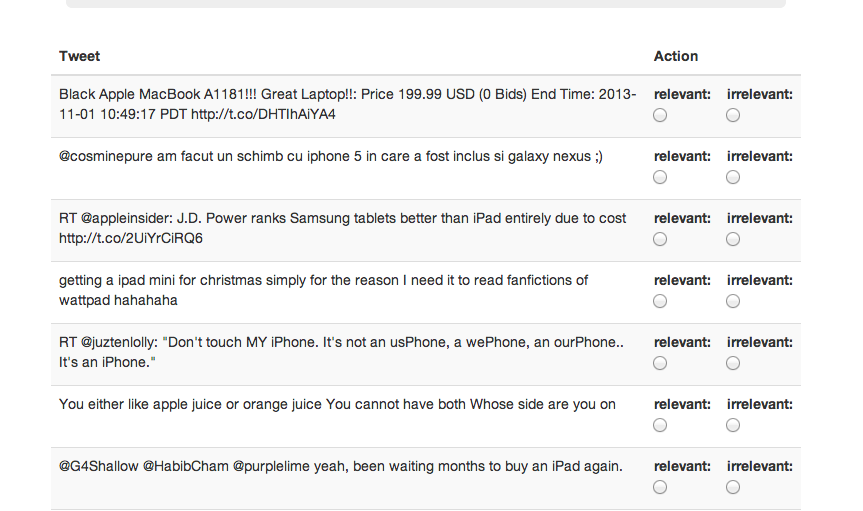
\includegraphics[scale=0.6]{figures/datalabeller}
  \end{center}
  \caption{The data labelling application}
\label{fig:labeller}
\end{figure}

Train data, also known as a training set is a set of data used to train a knowledge database, in
this case, a classifier. Our training set will be created by manually labelling a fraction of our
dataset. People write in different ways on Twitter and trying to create a new training set to
encompass all possibilities would be very time consuming and intractable. To make this process a
little easier, a web application for labelling tweets was created. \Figref{fig:labeller} is a
screen shot of what the application looks like.

\begin{figure}
  \begin{center}
    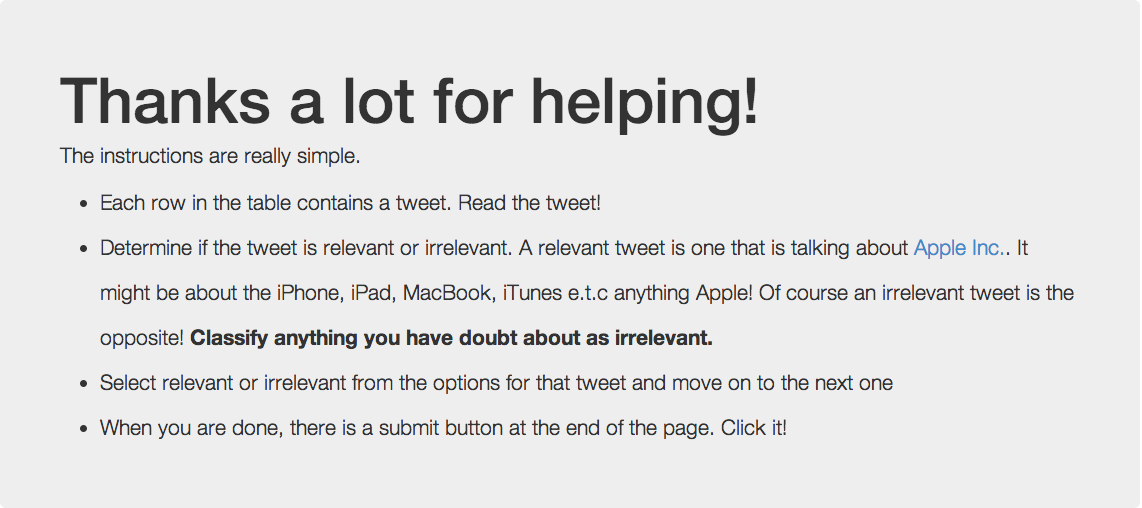
\includegraphics[scale=0.4]{figures/labeller_instructions}
  \end{center}
  \caption{Instructions on how to label the tweets}
\label{fig:labeller_instructions}
\end{figure}

While using the web application in \Figref{fig:labeller} makes labelling tweets easier and a
little quicker, it does not change the fact the we still have to manually label a plethora of
tweets. To speed up this process even further, the data labeller was made public and the labelling
was crowd sourced. A list of instructions (\Figref{fig:labeller_instructions}) were also given
to anyone who helped label the tweets.

One problem with crowd sourcing this task is that people have different opinions about what is
relevant and what is not. In an attempt to solve this problem, each tweet was classified twice. A
tweet classified as relevant gets a score of 1 and an irrelevant tweet gets 0. This means that if a
tweet was classified twice as relevant, it should have a score of 2 and a tweet classified as
irrelevant twice should have a score of 0. Tweets that have been classified twice and have a total
score of 1 are tweets that have been classified as both relevant and irrelevant. These are tweets
that we have to classify ourselves into a group. While this is not an assured way of getting the
best training set, it gives us a certain level of confidence about our training set. It is also
arguably much better than single handedly creating the training set.

\section{Training a classifier}
As discussed in Section~\ref{sec:bg_naive_bayes}, a Na\"{i}ve Bayes Classifier is a probabilistic
classifier which is based on the Bayes Theorem. We will train one and use it to classify the tweets
into relevant and irrelevant groups.

Unfortunately, the classifier takes as input a vector space representation of our tweets and not the
actual text. This means we have to convert our tweets into a vector representation of some sort. We
will be using the \textbf{bag of words model} in this study but before we transform the tweets, we
have to pre-process the tweets.

\subsection{Preprocessing}
\label{sec:preprocessing}
Preprocessing are the tasks we have to carry out before the main transformation of the tweets to a
vector space model. Firstly, we will peruse through our tweets to remove new line characters, links
and stop words. We then take each tweet and convert it into a list of \textit{n-grams}.

Some tweets have special characters like new lines, excess spaces and Unicode characters and these
characters are irrelevant for our use-case. Every programming language has a function to strip
off newlines and whitespace and it can be easily done in one line of code. Removing the links from
the text is a little more complex and the ``easiest'' way to do this would be to use a regular
expression. \citet{friedl2006mastering} in his book \textit{Mastering Regular Expressions} describes
regular expressions as a very flexible mini language that is used for text processing. The regular
expression we will be using to find links in our text is
\begin{verbatim}
  {(https?:\/\/)?([\da-z\.-]+)\.([a-z\.]{2,6})([\/\w \.-]*)*\/?}
\end{verbatim}

Unfortunately, all a regular expression can do is search for patterns in text. Luckily, most
programming languages provide support for regular expressions so all we have to do is search for the
pattern in each tweet and use the language features to replace the matched pattern with nothing(an
empty string preferably).

The next step is to remove stop words in each tweet. \citet{wilbur1992automatic} defines a stop word
as ``\textit{a word which may be identified as a word that has the same likelihood of occurring in
those documents not relevant to a query as in those documents relevant to the query.}'' In other
words, stop words occur in every document irrespective of the document's relevance. Stop words are
usually the most common word in a language, English in this case. Some examples include
\textit{and}, \textit{or}, \textit{the} etc. Removal of stop words from text usually results in
better model performance as shown in \Figref{fig:auc_curves_stopwords} on page
\pageref{fig:auc_curves_stopwords}.

%TODO: reference a table in a future section that proves this.

Finally, we convert each tweet to a list of \textit{n-grams}. An n-gram ``\textit{is a contiguous
sequence of n items from a given sequence of text}''\footnote{See
http://en.wikipedia.org/wiki/N-gram}. The easiest way to understand n-grams is with an example.
Assuming we have a document with the text ``machine learning rocks''. All unigrams(n-grams
where n is 1) that can be extracted from that text are \textit{``machine''}, \textit{``learning''}
and \textit{``rocks''}. Also, all bigrams(n-grams where n is 2) in the document are
\textit{``machine learning''} and \textit{``learning rocks''}. In this study, we will be using a
combination of unigrams and bigrams.

We have discussed different preprocessing tasks that we have to apply to our documents before
transforming them into the bag of words matrix representation. In the next section, we will look
into how the bag of words model works and then transform our tweets into this model.


\subsection{Transforming tweets to bag-of-words}
The bag of words model is a common representation for text that involves representing a document as
a multiset of its words. It is a very common way to represent documents and it has also been used
recently in computer vision \citep{sivic2009efficient}. All sets are combined to form a
document-term matrix of the corpora. The rows represent each document while the columns represent
the occurrence/frequency of a word in that document. To show how this works, let us assume we have
the following documents:
\begin{description}
  \item[A] today is a sunny day.
  \item[B] it is a sunny day isn't it?
  \item[C] what a sunny day!
\end{description}

\begin{table}
  \begin{center}
    \begin{tabular}{|c|c c c c c c c|}
      \hline
      & today & what & it & is & a & sunny & day \\
      \hline
      A & 1 & 0 & 0 & 1 & 1 & 1 & 1 \\
      B & 0 & 0 & 2 & 1 & 1 & 1 & 1 \\
      C & 0 & 1 & 0 & 0 & 1 & 1 & 1 \\
      \hline
    \end{tabular}
    \caption{A bag-of-words representation}
    \label{tab:document-term_matrix}
  \end{center}
\end{table}

By the above definition, \Tableref{tab:document-term_matrix} will be an accurate representation
of our sentences using the bag of words model. Note that in our example, each sentence is a document
and all sentences form the corpora.

Now that we have converted our corpora into a bag of words representation, we will now use the
resulting matrix to train our classifier.

\subsection{Training the initial classifier}
\begin{figure}
  \centering
  \begin{subfigure}[b]{0.49\linewidth}
    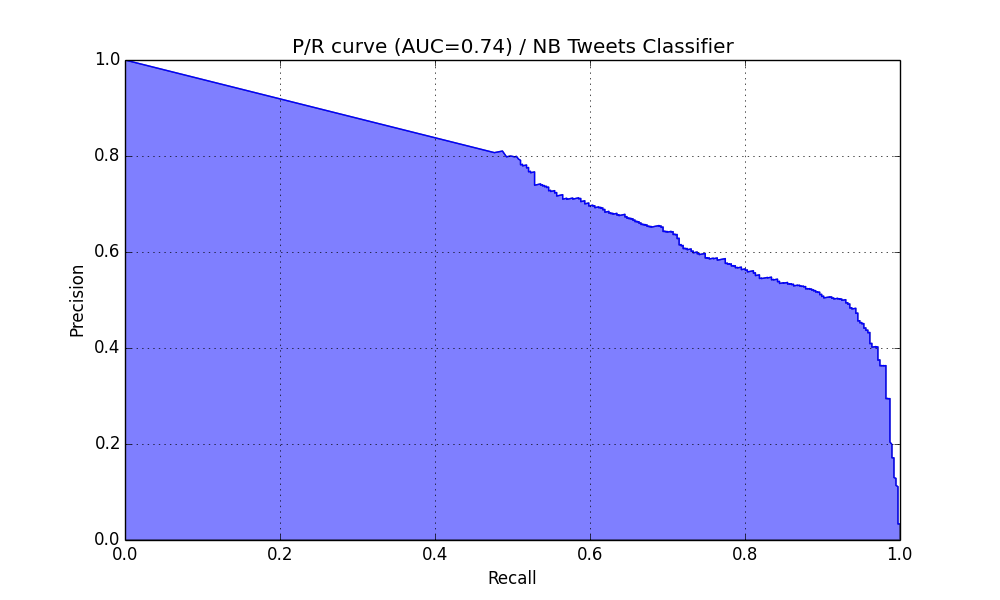
\includegraphics[width=\linewidth]{figures/pr_NB_Tweets_Classifier_01}
  \caption{AUC=74 with stopwords}
  \label{fig:auc_with_stopwords}
  \end{subfigure}
  % =============
  \begin{subfigure}[b]{0.49\linewidth}
      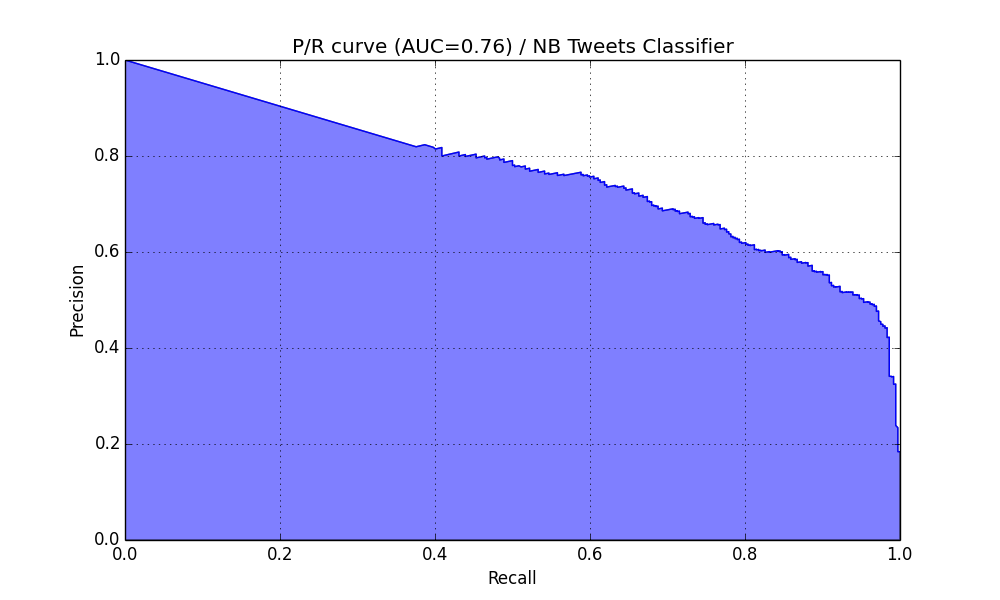
\includegraphics[width=\linewidth]{figures/pr_NB_Tweets_Classifier_02}
  \caption{AUC=76 without stopwords}
  \label{fig:auc_without_stopwords}
  \end{subfigure}

\caption{AUC curves with and without stopwords}
\label{fig:auc_curves_stopwords}
\end{figure}

\begin{table}
  \begin{subtable}{.5\linewidth}
    \centering
    \begin{tabular}{cccc} \toprule
      accuracy        & std($\sigma$) & AUC             & std($\sigma$) \\ \midrule
      0.9875          & 0.0000        & 0.7387          & 0.0000 \\
      0.9877          & 0.0002        & 0.7381          & 0.0000 \\
      \textbf{0.9878} & 0.0002        & 0.7312          & 0.0090 \\
      0.9877          & 0.0002        & 0.7412          & 0.0190 \\
      \textbf{0.9878} & 0.0002        & 0.7454          & 0.0190 \\ \midrule
      0.9876          & 0.0005        & 0.7394          & 0.0220 \\
      0.9875          & 0.0005        & 0.7431          & 0.0220 \\
      0.9874          & 0.0005        & 0.7427          & 0.0200 \\
      0.9874          & 0.0005        & \textbf{0.7455} & 0.0210 \\
      0.9873          & 0.0005        & 0.7454          & 0.0200 \\ \bottomrule
    \end{tabular}
      \caption{With stopwords}
      \label{tab:data_with_stopwords}
  \end{subtable}
  % =======================
  \begin{subtable}{.5\linewidth}
    \centering
    \begin{tabular}{cccc} \toprule
      accuracy        & std($\sigma$) & AUC             & std($\sigma$) \\ \midrule
      \textbf{0.9908} & 0.0000        & 0.7526          & 0.0000 \\
      0.9904          & 0.0004        & 0.7589          & 0.0060 \\
      0.9903          & 0.0003        & 0.7485          & 0.0150 \\
      0.9901          & 0.0004        & 0.7535          & 0.0160 \\
      0.9901          & 0.0003        & 0.7572          & 0.0160 \\ \midrule
      0.9901          & 0.0003        & 0.7582          & 0.0150 \\
      0.9902          & 0.0004        & \textbf{0.7618} & 0.0160 \\
      0.9901          & 0.0004        & 0.7587          & 0.0170 \\
      0.9901          & 0.0004        & 0.7592          & 0.0160 \\
      0.9900          & 0.0004        & 0.7572          & 0.0160 \\ \bottomrule
    \end{tabular}
      \caption{Without stopwords}
      \label{tab:data_without_stopwords}
  \end{subtable}
\caption{Tables showing accuracy and AUC for 10-fold cross validation}
\label{tab:all_data_tables}
\end{table}



\subsection{Improving the classifier}
\begin{figure}
  \centering
  \begin{subfigure}[b]{0.49\linewidth}
    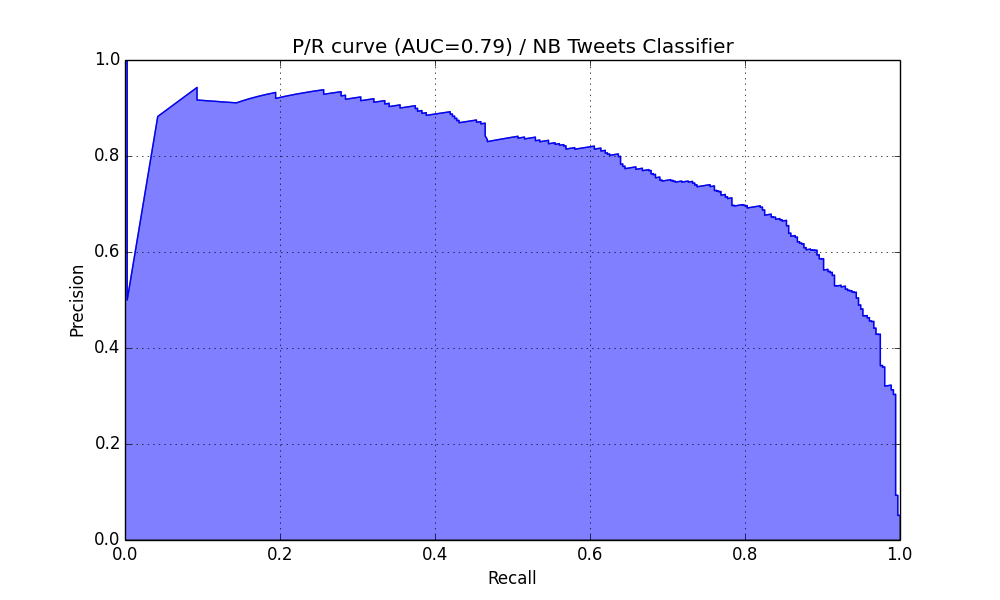
\includegraphics[width=\linewidth]{figures/pr_NB_Tweets_Classifier_03}
  \caption{AUC curve for tf-idf weighted corpora}
  \label{fig:auc_tfidf}
  \end{subfigure}
  % =============
  \begin{subfigure}[b]{0.49\linewidth}
    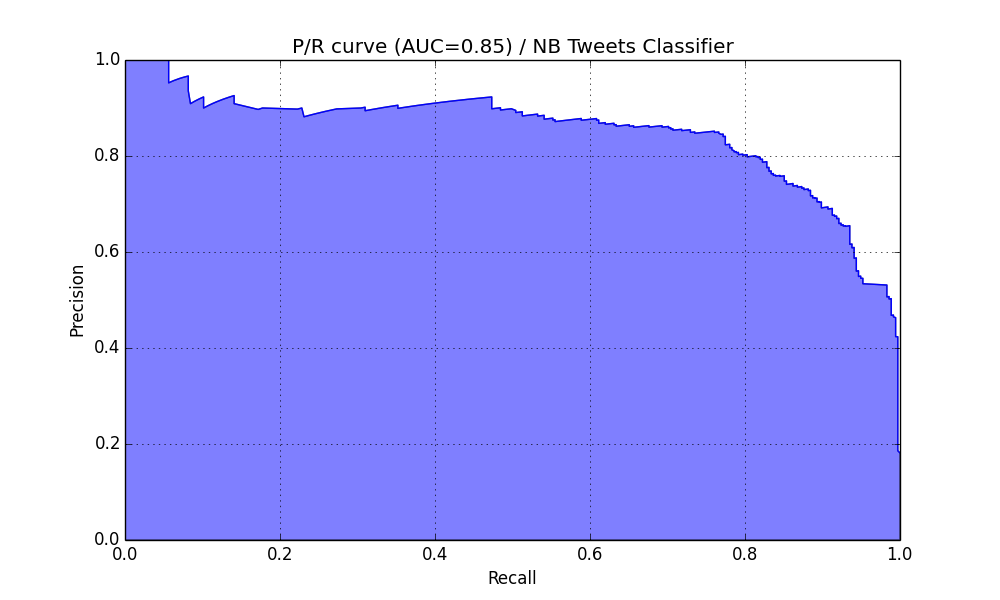
\includegraphics[width=\linewidth]{figures/pr_NB_Tweets_Classifier_04}
  \caption{AUC curve for best found model}
  \label{fig:auc_best_model}
  \end{subfigure}

  \caption{AUC curves for tf-idf weighted and best found models, resectively}
  \label{fig:auc_curves_tfidf_grid}
\end{figure}


\begin{table}
  \begin{subtable}{.5\linewidth}
    \centering
    \begin{tabular}{cccc} \toprule
      accuracy & std($\sigma$) & AUC    & std($\sigma$) \\ \midrule
      0.9939   & 0.0000        & 0.8068 & 0.0000 \\
      0.9939   & 0.0000        & 0.8006 & 0.0062 \\
      0.9949   & 0.0001        & 0.7893 & 0.0167 \\
      0.9939   & 0.0003        & 0.7960 & 0.0186 \\
      0.9939   & 0.0003        & 0.7892 & 0.0215 \\ \midrule
      0.9939   & 0.0004        & 0.7920 & 0.0206 \\
      0.9939   & 0.0004        & 0.7902 & 0.0196 \\
      0.9939   & 0.0004        & 0.7900 & 0.0183 \\
      0.9939   & 0.0004        & 0.7890 & 0.0175 \\
      0.9939   & 0.0004        & 0.7876 & 0.0171 \\ \bottomrule
    \end{tabular}
      \caption{With stopwords}
      \label{tab:data_with_stopwords}
  \end{subtable}
  % =======================
  \begin{subtable}{.5\linewidth}
    \centering
    \begin{tabular}{cccc} \toprule
      accuracy & std($\sigma$) & AUC    & std($\sigma$) \\ \midrule
      0.9961   & 0.0000        & 0.8415 & 0.0000 \\
      0.9960   & 0.0001        & 0.8610 & 0.0195 \\
      0.9955   & 0.0007        & 0.8445 & 0.0282 \\
      0.9955   & 0.0006        & 0.8491 & 0.0257 \\
      0.9954   & 0.0005        & 0.8441 & 0.0251 \\ \midrule
      0.9954   & 0.0005        & 0.8447 & 0.0229 \\
      0.9954   & 0.0005        & 0.8465 & 0.0217 \\
      0.9954   & 0.0004        & 0.8470 & 0.0203 \\
      0.9954   & 0.0004        & 0.8468 & 0.0192 \\
      0.9954   & 0.0004        & 0.8487 & 0.0191 \\ \bottomrule
    \end{tabular}
      \caption{Without stopwords}
      \label{tab:data_without_stopwords}
  \end{subtable}
\caption{Tables showing accuracy and AUC for 10-fold cross validation}
\label{tab:all_data_tables}
\end{table}

\chapter{Topic Modelling}
\label{cha:topic_modelling}
In this chapter, we use a topic model to find themes/topics that exist in our dataset. Our input
dataset is a set of relevant tweets as determined by the classifier in the previous chapter. We use
Latent Dirichlet Allocation as our topic model as described in \Sectionref{sec:bg_lda} on page
\pageref{sec:bg_lda}.

Tables~\ref{tab:30-topics} and~\ref{tab:40-topics} on pages \pageref{tab:30-topics} and
\pageref{tab:40-topics} each show a list of 30 and 40 topics. It also contains their respective
topic-tokens distribution. For the purpose of this study, a token is either a unigram or bigram.
Each row comprises of a list of tokens that try to explain a topic and they are ordered by their
level of influence. While it is helpful to have our tokens ordered by level of influence, the
respective influence values are excluded from the table because we will not pay much
attention to them during our analysis.

% TODO: Briefly explain methodology of analysis

\section{Preprocessing}
\label{sec:lda_preprocessing}
% TODO: Complete this section

\section{Evaluating Topic Models}
\label{sec:evaluating_topic_models}
In this section, we analyse two separate models one of which will comprise of 30 topics while the
other of 40 topics. They both use a mixture of unigrams and bigrams in their token distribution.
This was inspired by our experiments in \Sectionref{sec:training_classifier} where the classifier
showed better performance when using a mixture of unigrams and bigrams. We analyse a few topics for
each model and have a look at some of the tweets that fall under those topics.
% TODO: Something about our empirical approach to the evaluation here

\subsection{Evaluating 30 Topics}
\label{sec:evaluating-30-topics}
\begin{figure}
\begin{center}
  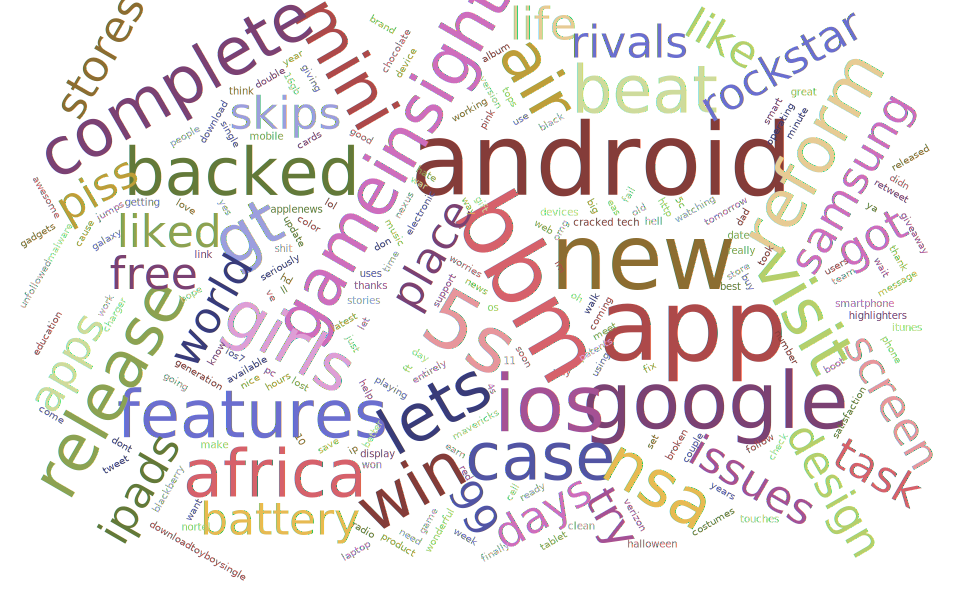
\includegraphics[scale=0.75,angle=90]{Figures/30_topics_cloud}
\end{center}
\caption{A word cloud of all tokens from all topics in our 30-topics model}
\label{fig:30-topics-cloud}
\end{figure}

The topic-word distributions in \Tableref{tab:30-topics} are a combination of unigrams
and bigrams.\\

\begin{longtable}{c p{16cm}} \toprule
  Topic & Topic-Tokens Distribution \\ \midrule
   0    & app, latest, generation, version, galaxy, won, set, oh, save, minute \\ \midrule
   1    & walk, watching, unveils, today stories, beat rivals, ipads beat, missed unveils, revamped, revamped ipads, rivals \\ \midrule
   2    & perfect, case, 16gb, black, gt, giving, clean, smartphone, ya, pink \\ \midrule
   3    & screen, place, http, better, place visit, visit gameinsight, entirely, electronic \\ \midrule
   4    & video, love, app android, yay, tomorrow, let, liked, liked video, operating, single \\ \midrule
   5    & complete, follow, managed, week, having, girls, task, complete task, managed complete \\ \midrule
   6    & ios, lets, bbm ios, ios lets, lets apps, features, game, tech, missed \\ \midrule
   7    & google, backed, google samsung, mobile, nortel, patents, microsoft backed, rockstar, backed rockstar, uses \\ \midrule
   8    & using, world, best, hate, beat, skips, skips africa, africa, africa world, release 5s \\ \midrule
   9    & music, 10, mavericks, number, yes, coming, soon, earn, cards, support \\ \midrule
   10   & new, app, store, available, design, playing, stargazing, stargazing app, new design \\ \midrule
   11   & really, os, gift, stores, hours, news, fail, stores piss, piss, broken \\ \midrule
   12   & day, battery, good, shit, display, thanks, battery life, omg, seriously, ios7 \\ \midrule
   13   & android, use, blackberry, update, web, 11, issues, devices, hd, fix issues \\ \midrule
   14   & official, 5s, 5c, life, models, cracked, color, worries, nexus, highlighters \\ \midrule
   15   & know, pc, 4s, old, does, releases, air saywhatnow, releases air, saywhatnow, did \\ \midrule
   16   & time, ll, date, wonderful, charger, working, nice, message, cell, took \\ \midrule
   17   & got, today, ve, going, smart, help, protector, hell, screen protector, got new \\ \midrule
   18   & samsung, don, download, updated, people, radio, meet, ft, updated ios, malware jumps \\ \midrule
   19   & nsa, microsoft, facebook google, google substantial, nsa surveillance, reform, reform nsa, substantial, substantial reform, surveillance \\ \midrule
   20   & lol, education, chocolate, team, double, wait, boot, white girls, girls like, couple days \\ \midrule
   21   & air, free, visit, power, satisfaction, 99 free, app 99, power tablet, tops, war \\ \midrule
   22   & release, like, new, facebook, big, make, new 5s, gadgets, product, brand \\ \midrule
   23   & just, white, app, gold, users, gold 5s, awesome, way, unfollowed, link \\ \midrule
   24   & verizon, laptop, finally, say, dont, years, getting, ready, costumes, lost \\ \midrule
   25   & apps, phone, check, ip, cause, thank, hope, dad, im, gt gt \\ \midrule
   26   & gameinsight, halloween, try, retweet, giveaway, win, work, try gameinsight, days, tweet \\ \midrule
   27   & bbm, bbm android, official release, android official, android bbm, perfect features, features bbm, want, buy, need \\ \midrule
   28   & mini, win, chance, come, chance win, case mini, kickstand, kickstand case, mini models \\ \midrule
   29   & itunes, released, think, year, great, touches, album, downloadtoyboysingle, didn, eas \\ \bottomrule
\caption{30 topic-tokens distribution with unigrams and bigrams}
\label{tab:30-topics}
\end{longtable}
%analyse 6, 7, 9, 12, 13, 14, 22, 27, 28



\subsubsection{Topic 6}
\label{sec:topic_6}
\textit{ios, lets, bbm ios, ios lets, lets apps, features, game, tech, missed} \\\\
The most common theme in the above distribution is ``ios'' and ``lets''. ``bbm'' also seems to have
a considerate amount of relevancy as it is the third most relevant token. The other tokens seem
random but we should be able to explain them better after taking a look at some of the tweets with a
fair proportion of this topic.

\begin{table}[H]
  \begin{tabular}{c c p{13cm}} \toprule
    No & Proportion & Tweet \\ \midrule
    1  & 81\%       & Fantastical 2 for iPhone gets bold iOS 7 redesign, many new features \#tech \\ \midrule
    2  & 75\%       & Limbo for iOS is now even cheaper at \$0.99 \\ \midrule
    3  & 80\%       & Don't miss out on loads of great iOS game sales from\ldots \\ \midrule
    4  & 70\%       & What new features does Apple's iOS 7 boast? \\ \midrule
    5  & 63\%       & get the BBM on iPhone iOS, lets get the apps here now \\ \midrule
    6  & 89\%       & time guessing is hard! test yourself on ur iPhone it's \#cool tweet your
    results from the app \#game \#ios \#app \\ \bottomrule
  \end{tabular}
  \caption{Tweets classified under topic 6}
  \label{tab:topic_6_tweets}
\end{table}

The tweets in \Tableref{tab:topic_6_tweets} all seem to have at least 63\% of topic 6. While they
might look like carefully selected tweets, they were actually chosen at random. Our dataset contains
a large fraction of the third, fourth and fifth tweet. Approximately 90\% of them are retweets which
explains why our topic model extracted ``ios lets'', ``lets apps'', ``game'' and ``tech'' as
relevant tokens. The sixth tweet arguably does not really have anything to do with ``iOS'' but
because it has been tagged with three words that our topic model finds salient, it gets tagged as
having 89\% proportion of topic 6.



\subsubsection{Topic 7}
\label{sec:topic_7}
\textit{google, backed, google samsung, mobile, nortel, patents, microsoft backed, rockstar, backed
rockstar, uses } \\\\
From a simple scan through the tokens in this topic, we can postulate that the tweets in this topic
will mostly be about Google, Samsung, Nortel and the Rockstar Consortium. Nortel was a
communications and networking equipment manufacturer which went bankrupt and the Rockstar Consortium
was formed to negotiate licensing for patents they owned. However, we do not expect our whole
dataset to be about patent war between these companies. Samsung and Google are large technology
companies and we might encounter tweets that simple compare their products with that of Apple. We
can make this assumption because we know our dataset is Apple-centric.

\begin{table}[H]
  \begin{tabular}{c c p{13cm}} \toprule
    No  & Proportion & Tweet \\ \midrule
    1   & 86\%       & Apple files patent for slim solar-powered technology via GigaOM \\ \midrule
    2   & 78\%       & Google, Samsung, and others sued over search patents by Apple-backed Nortel group \\ \midrule
    3   & 78\%       & Apple, Microsoft-Backed Rockstar Consortium Sues Google, Samsung Over 7 \\ \midrule
    4   & 83\%       & Apple, Microsoft-backed Rockstar uses Nortel patents to sue Google, Samsung and others \\ \midrule
    5   & 78\%       & Google Fiber comes to iPhone, iPod touch with DVR functions \\ \midrule
    6   & 80\%       & Google Replacing Android ID With Advertising ID Similar To Apple's IDFA \\ \midrule
    7   & 68\%       & Nexus 4 will get the updated ``in the coming weeks''. If Apple can offer to update the (almost) entire install base on day 1, why not Google? \\ \midrule
    8   & 88\%       & Google smartwatch: Will it be an ``iPhone'' moment for wearables? \\ \midrule
    9   & 84\%       & I wonder who's richer Google or Apple?! \\ \midrule
    10  & 90\%       & Apple earned more than Samsung, LG, Nokia, Huawei, Lenovo \& Motorola's mobile shipments combined \\ \bottomrule
  \end{tabular}
  \caption{Tweets classified under topic 7}
  \label{tab:topic_7_tweets}
\end{table}

\Tableref{tab:topic_7_tweets} is a list of 10 randomly selected tweets with with a fair proportion
of our topic. The first four tweets are about patents and lawsuits and our dataset contains a number
of variations of those tweets, each of which have been retweeted many times. The fifth, sixth and
seventh tweets all talk about products by Google while the last three tweets compare Apple's
products to that of other companies.


\subsubsection{Topic 9}
\label{sec:topic_9}
\textit{music, 10, mavericks, number, yes, coming, soon, earn, cards, support}\\\\
This topic, compared to previous topics, is a little tougher to analyse. ``music'' is th most
salient token in the distribution but we also have unrelated tokens like ``mavericks'', ``cards'',
``earn'' and ``support''. While they might actually be closely related, it is not very obvious that
they are by merely looking at the topic-token distribution. To get a better understanding of this
topic, we take a look at some tweets with a fair proportion of the topic.

\begin{table}[H]
  \begin{tabular}{c c p{13cm}} \toprule
    No & Proportion & Tweet \\ \midrule
    1  & 63\%       & Just updated my mac - in loveee \#Mavericks \\ \midrule
    2  & 83\%       & nahhhh, save up some cash to buy that freaking iPhone 6 thats coming out soon :) \\ \midrule
    3  & 77\%       & iPhone Battery Always Running Low? 10 Tips To Prolong The Battery Life. \\ \midrule
    4  & 70\%       & I wish I could type my mood into my iPhone and it would make a playlist for me. \\ \midrule
    5  & 67\%       & I would like to tag items on my iPhone and then be able to search tags, like in Mavericks. \\ \midrule
    6  & 75\%       & Apple needs to make a iPhone thats bigger than 64gb! My music has just about filled mine \\ \midrule
    7  & 70\%       & iPhone has to let me record videos while music playing on my phone. LET ME BE GREAT APPLE!!! \\ \midrule
    8  & 76\%       & if you have an iPhone you can block the number \\ \midrule
    9  & 58\%       & My phone just erased everybody messages number with an iPhone. \\ \midrule
    10 & 78\%       & Earn gift cards, flier miles and more with Perk - download for iphone now! \\ \bottomrule
  \end{tabular}
  \caption{Tweets classified under topic 9}
  \label{tab:topic_9_tweets}
\end{table}

Apple released a new operating system called Mavericks around the time our dataset was gathered
which is what the first and fifth tweets are about in \Tableref{tab:topic_9_tweets} and it also
explains what the token ``mavericks'' means. The second tweet talks about the arrival of an iPhone 6
but our dataset only contains less than 10 tweets with the word ``coming''. Tweets 4, 6 and 7 all
talk about music and our dataset contains a large amount of those type of tweets while tweets 8 and
9 talk about mobile numbers. Without having to dig deeper, it is obvious that our topic is not well
formed as it is a combination of multiple topics that do not complement each other.

\subsubsection{Topic 12}
\label{sec:topic_12}
\textit{day, battery, good, shit, display, thanks, battery life, omg, seriously, ios7}\\\\
The most salient token we have is ``day'' which does not mean much to us. Our token-distribution
also seems to have a number of adverbs, adjectives and slang like ``good'', ``seriously'' and
``omg''. These all seem to represent sentiments towards a certain topic. Ignoring them, we are left
with ``thanks'', ``battery'' and ``battery life''. At this point, we could postulate that most of
the tweets in this category will have a ``battery'' theme. To confirm this, we take a look at some
of the tweets with a fair proportion of the topic.

\begin{table}[H]
  \begin{tabular}{c c p{13cm}} \toprule
    No & Proportion & Tweet \\ \midrule
    1  & 81\%       & iPhone battery just went from 23\% to 3\% in the space of five minutes. Thanks again, iOS7. \\ \midrule
    2  & 76\%       & iPhone battery is so crap \\ \midrule
    3  & 80\%       & iPhone battery dropping in 5\% increments. Can't be a good sign. \\ \midrule
    4  & 64\%       & Considering the amount of times I have to plug my IPhone in to charge a day it might as well be a fucking landline \\ \midrule
    5  & 50\%       & FORGOT MY IPHONE CHARGER oh shit man. My poor battery :( \\ \midrule
    6  & 66\%       & Apple was considering making an iPod for kids but apparently, the name iTouch Kids didn't sit too well. \\ \midrule
    7  & 50\%       & so your apple store doesn't get stock on release day? \\ \midrule
    8  & 50\%       & can I have an iphone with bbm and the battery life of a nokia please \\ \bottomrule
  \end{tabular}
  \caption{Tweets classified under topic 12}
  \label{tab:topic_12_tweets}
\end{table}

All tweets(except the 7th) in \Tableref{tab:topic_12_tweets} all refer to the iPhone battery life. A
very large number of tweets that have a good proportion of this topic take in some way, the shape of
tweets 1--4 in our table and fortunately, our topic model is able to find the relationship between
these tweets.

The seventh tweet looks out of place as it has nothing to do with battery life but
going back to our topic-token distribution, the most salient token as described by the model is
``day''. Luckily, our dataset also contains a large number of that tweet. This is because that
articular tweets was retweeted a lot of times.


\subsubsection{Topic 13}
\label{sec:topic_13}
\textit{android, use, blackberry, update, web, 11, issues, devices, hd, fix issues}\\\\
At first glance, the main themes that stand out in the above distribution are ``android'',
``blackberry'' and ``issues''. Our dataset is Apple-centric so we could assume that the tweets with
a large proportion of this topic will have some sort of comparison between Apple, Android and
Blackberry with respect to issues that occur with their products. If this is not the case, it is
possible that our topic model has merged two different topics into one topic. To verify our
assumption, we analyse a few tweets that have a reasonable proportion of this topic.

\begin{table}[H]
  \begin{tabular}{c c p{13cm}} \toprule
    No & Proportion & Tweet \\ \midrule
    1  & 51\%       & Wow hello typos\ldots cracked iphone screen problems \\ \midrule
    2  & 50\%       & Check out WhatsApp Messenger for BlackBerry, Android, iPhone, Nokia and Windows Phone. Download it today from\ldots \\ \midrule
    3  & 50\%       & Pandora finally comes to Chromecast via Android and iPhone apps \\ \midrule
    4  & 80\%       & I just connected with friends on \#BBM\@. Invite your BlackBerry, Android and iPhone friends at\ldots \\ \midrule
    5  & 80\%       & Develop iPhone, Ipad and Android Apps creatively with Mawaqaa. \\ \midrule
    6  & 75\%       & Was curious if that was the culprit. I have had tons of issues since upgrading my Apple devices to latest \\ \midrule
    7  & 57\%       & Apple testing Mail update for OS X Mavericks to fix several issues \\ \midrule
    8  & 78\%       & Manufacturing issue causing battery problems in some iPhone 5s devices \\ \bottomrule
  \end{tabular}
  \caption{Tweets classified under topic 13}
  \label{tab:topic_13_tweets}
\end{table}

Tweets 2--5 in \Tableref{tab:topic_13_tweets} all have either an android or blackberry theme in them
which is expected. They all talk about applications on all three platforms. On the other hand,
tweets 1, 6, 7 and 8 all have an ``issues'' theme in them. Unfortunately, these two topics do not
really complement each other and should arguably be splitted into two separate topics. Some of the
latter mentioned tweets do also talk about applications on Apple's platforms which may be the reason
why our topic model observed a relationship between these topics.



\subsubsection{Topic 14}
\label{sec:topic_14}
\textit{official, 5s, 5c, life, models, cracked, color, worries, nexus, highlighters}\\\\

\begin{table}[H]
  \begin{tabular}{c c p{13cm}} \toprule
    No & Proportion & Tweet \\ \midrule
    1  & 88\%       & Cracked iPhone No worries. Color it in with highlighters! \\ \midrule
    2  & 68\%       & Apple discovers manufacturing defect causing iPhone 5S battery woes for some customers \\ \midrule
    3  & 88\%       & \#Apple Admits Defect with Some \#iPhone 5s Batteries \\ \midrule
    4  & 33\%       & Everyone who bought the iPhone 5S or iPhone 5C is dumb. The iPhone 6 has already been announced lol. \\ \midrule
    5  & 76\%       & iPhone 5S, 5C debut in India today - Customers get the new models in the price range of Rs 41,900 to Rs 71,500 \\ \midrule
    6  & 88\%       & \$AAPL Apple's yellow iPhone 5C is a lemon \\ \midrule
    7  & 51\%       & Well the battery life on the iPhone 5c is great\ldots I need a charger in every room \\ \midrule
    8  & 22\%       & What Are The Most Popular iPhone 5s and 5c Colors? Space Gray And Blue. \\ \bottomrule
  \end{tabular}
  \caption{Tweets classified under topic 14}
  \label{tab:topic_14_tweets}
\end{table}



\subsubsection{Topic 22}
\label{sec:topic_22}
\textit{release, like, new, facebook, big, make, new 5s, gadgets, product, brand}\\\\

\begin{table}[H]
  \begin{tabular}{c c p{13cm}} \toprule
    No & Proportion & Tweet \\ \midrule
    1  & \%       & \\ \midrule
    2  & \%       & \\ \midrule
    3  & \%       & \\ \midrule
    4  & \%       & \\ \midrule
    5  & \%       & \\ \midrule
    6  & \%       & \\ \midrule
    7  & \%       & \\ \midrule
    8  & \%       & \\ \bottomrule
  \end{tabular}
  \caption{Tweets classified under topic 22}
  \label{tab:topic_22_tweets}
\end{table}



\subsubsection{Topic 27}
\label{sec:topic_27}
\textit{bbm, bbm android, official release, android official, android bbm, perfect features,
features bbm, want, buy, need} \\\\
At first glance, we could say this topic has a lot to do with \textit{android}, \textit{bbm}, and
\textit{features}. The last three tokens also seem out of place. At the time of data gathering,
there was a lot of chatter on social media about the BlackBerry Messenger(BBM) application coming to
the iOS and android platform. To be certain of this, let's take a look at some of the tweets that
have a fair proportion of this topic.

\begin{table}[H]
  \begin{tabular}{c c p{13cm}} \toprule
    No & Proportion & Tweet \\ \midrule
    1  & 56\%       & More perfect features, BBM android, BBM iPhone \\ \midrule
    2  & 50\%       & BBM on android and iPhone, official release - get it here \\ \midrule
    3  & 50\%       & BBM Now on Android and iPhone. \\ \midrule
    4  & 72\%       & Just got bbm chat for the iPhone, feel free to add me if you want :) \\ \midrule
    5  & 60\%       & Apple should create the option of removing yourself from a group chat \\ \midrule
    6  & 68\%       & Anyone want to buy a black 64GB ipad 2 from me in excellent condition? \\ \midrule
    7  & 25\%       & someone buy me an iphone ugh \\ \midrule
    8  & 76\%       & I need a iphone 5 asap \\ \bottomrule
  \end{tabular}
  \caption{Tweets classified under topic 27}
  \label{tab:topic_27_tweets}
\end{table}

\Tableref{tab:topic_27_tweets} is a list of tweets that fall under topic 27. We can see that the
first four tweets have a lot to do with the new BBM for iOS and Android. The fifth tweet is a little
tricky as it says nothing about BBM\@. However, it does in fact talk about a chat application which is
what BBM is. While the user might not have been referring to BBM in particular, our model was able
to pickup on the relationship between both subjects.

The last three tweets in our table explain the last three tokens in out topic-word distribution for
topic 27. This means that topic 27 is actually a combination of two different topics.



\subsubsection{Topic 28}
\label{sec:topic_28}
\textit{mini, win, chance, come, chance win, case mini, kickstand, kickstand case, mini models}\\\\
There are a lot of promotions/giveaways on Twitter that involve apple products. Tokens like
``win'', ``chance'' and ``chance win''  in our distribution tell us that this topic is about these
promotions. Our dataset is Apple-centric so we could hypothesise that tweets with a large proportion
of this topic might be offering users a chance to win Apple products like the iPad/Mac Mini, hence
the ``mini'' in our distribution. We also have ``case'' occurring in the distribution which might
refer to iPad cases up for promotion. To confirm that our hypothesis is valid, or not, we
analyse some tweets with a fair proportion of this topic.

\begin{table}[H]
  \begin{tabular}{c c p{13cm}} \toprule
    No & Proportion & Tweet \\ \midrule
    1  & 75\%       & Win an \$800 Mac Mini for FREE from MacTrast the perfect addition to any home or office! \\ \midrule
    2  & 82\%       & RT to WIN! - \#Win an iPad Mini to celebrate the start of \#50at50 \\ \midrule
    3  & 56\%       & 15,000 Facebook Fan Giveaway happening now - Win a Lens, iPad Mini, \$500 Amazon gift card and LOTS more! \#colorvale15k \\ \midrule
    4  & 94\%       & WIN an iPad mini plus a chance to win a Williamson Tea Elephant Tea Caddie \\ \midrule
    5  & 67\%       & Win an \#ipad follow and RT for a chance to win \\ \midrule
    6  & 66\%       & Targus Kickstand Case for Apple iPad Mini all models - Red \\ \midrule
    7  & 86\%       & Cooper Dynamo Apple iPad Mini Kids Play Case review \\ \midrule
    8  & 78\%       & Fab Purse Moschino IPhone Cases. Come in Lots of Colours \\ \midrule
    9  & 50\%       & Retina iPad Mini may be launched Nov. 21 \\ \midrule
    10 & 20\%       & iMore -- iMore show 373: iPad Air and Retina iPad mini buyers guide \\ \midrule
  \end{tabular}
  \caption{Tweets classified under topic 28}
  \label{tab:topic_28_tweets}
\end{table}

From \Tableref{tab:topic_28_tweets}, we can tell that Tweets 1--5 are all promotional tweets
offering users a chance to win Apple products like the iPad mini. 60\% of the tweets with a fair
proportion of this topic are all variations of those tweets. Tweets 6--8 all refer to iPad and
iPhone cases and contrary to what we previously assumed, these cases are not part of the promotion.
This means that our topic model has merged two topics that do not complement each other. The last
two tweets are also have nothing to do with the promotions as well as the cases. These tweets are
general tweets about the iPad mini. Fortunately, our topic model has tagged them with low
proportions(50\% and 20\% respectively) which is acceptable.



\subsection{Evaluating 40 Topics}
\label{sec:evaluating-40-topics}
% TODO: Complete this section

\begin{figure}
\begin{center}
  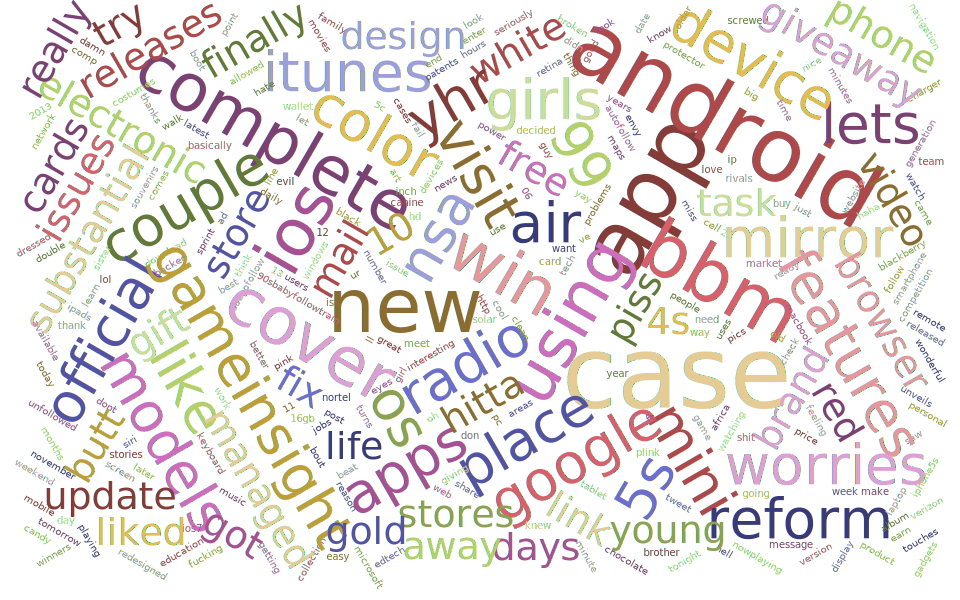
\includegraphics[scale=0.75,angle=90]{Figures/40_topics_cloud}
\end{center}
\caption{A word cloud of all tokens from all topics in our 40-topics model}
\label{fig:40-topics-cloud}
\end{figure}

\begin{longtable}{c p{16cm}} \toprule
  Topic & Topic-Words associations \\ \midrule
   0    & big, year, chocolate, mobile, gadgets, double, boot, girls like, white girls, touches \\ \midrule
   1    & app, store, know, available, does, design, stargazing, stargazing app, ft, new design \\ \midrule
   2    & gift, version, 25, liked, liked video, months, earn, watch, gift cards, knew \\ \midrule
   3    & follow, ip, place, walk, laptop, electronic, web, dont, competition, costumes \\ \midrule
   4    & using, hate, tweet, using app, reason, bout, thing, unfollowed using, case like, girl \\ \midrule
   5    & white, education, giveaway, tablet, comes, brand, brand new, way, halloween giveaway, win plink \\ \midrule
   6    & visit, place visit, visit gameinsight, ipads, place, unveils, power, rivals, stories case \\ \midrule
   7    & video, download, 16gb, black, watching, nowplaying, clean, smartphone, eyes, sprint \\ \midrule
   8    & great, giving, yay, miss, post, feeling, turns, maps, keyboard, canine evil \\ \midrule
   9    & number, tfbjp teamfairyrose, retweet tfbjp, sougofollow, teamfairyrose, autofollow, 06, cards, 90sbabyfollowtrain, interesting \\ \midrule
   10   & ios, official, 5s, like, world, game, facebook, new 5s, cool, africa \\ \midrule
   11   & new, gameinsight, try, updated, try gameinsight, achievement, new achievement, jobs, achievement 10, areas \\ \midrule
   12   & android, need, use, blackberry, devices, hd, problems, card, art, issue \\ \midrule
   13   & bbm, bbm android, official release, android official, got, want, gold, macbook, gold 5s, smart \\ \midrule
   14   & apps, lets, bbm ios, ios lets, lets apps, phone, don, best, people, meet \\ \midrule
   15   & missed, having, app android, case missed, windows, 12, daily, cell, apps android, decided \\ \midrule
   16   & perfect, android bbm, perfect features, features bbm, love, collection, pink, did, let, website \\ \midrule
   17   & samsung, google samsung, backed, entirely, nortel, patents, share, beat, uses, really entirely \\ \midrule
   18   & mini, win, chance, chance win, models red, kickstand case, mini models, targus, targus kickstand, case mini \\ \midrule
   19   & air, http, better, young, news, mirror, market, mirror world, souvenirs mirror, envy complete \\ \midrule
   20   & retina, device, red, electronic device, device using, ur, inch, 13, fix, wallet \\ \midrule
   21   & pc, life, old, releases, saywhatnow, releases air, air saywhatnow, cases, away, battery life \\ \midrule
   22   & check, music, 10, mavericks, generation, os mavericks, ready, fix issues, mail, mail update \\ \midrule
   23   & case, buy, cover, 99, end, 2013, case 4s, case cover, smart cover, cover case \\ \midrule
   24   & haha, isn, line, allowed, oh, solar, price, android phone, guy, basically \\ \midrule
   25   & app, just, radio, updated ios, users, young hitta, yhr app, yhr, radio yhr, hitta radio \\ \midrule
   26   & os, stores, playing, latest, hours, fail, piss, stores piss, issues, protector \\ \midrule
   27   & release, halloween, 5c, work, models, days, online, product, color, pics \\ \midrule
   28   & battery, lol, good, shit, thanks, tomorrow, ios7, minutes, minute, november \\ \midrule
   29   & itunes, released, think, thank, album, downloadtoyboysingle, itunes link, downloadtoyboysingle itunes, saw, sister \\ \midrule
   31   & ll, charger, didn, personal, later, nice, brother, movies, butt, butt away \\ \midrule
   32   & features, tech, make, cracked, worries, color highlighters, cracked worries, highlighters, worries color, say \\ \midrule
   33   & complete, 4s, , managed, week, display, girls, task, managed complete, complete task \\ \midrule
   34   & free, enter, win, 99 free, app 99, iphone5s, navigation, comp, fucking, network \\ \midrule
   35   & really, update, broken, damn, 11, family, seriously, point, message, took \\ \midrule
   36   & time, retweet, date, wonderful, hell, edtech, learn, screwed, winners chosen, chosen tonight \\ \midrule
   36   & today, ve, going, verizon, couple, couple days, team couple, dressed, came, online store \\ \midrule
   37   & screen, finally, look, years, getting, weekend, remote, siri, finally got, ad redesigned \\ \midrule
   38   & google, nsa, microsoft, reform, reform nsa, substantial, substantial reform, surveillance, facebook google, nsa surveillance \\ \midrule
   39   & day, easy, link, older, candy, browser, os browser, otterbox, defender, otterbox defender \\ \bottomrule
\caption{40 word-topic distributions with unigrams and bigrams}
\label{tab:40-topics}
\end{longtable}



% \chapter{Further Analysis}
\label{cha:further_analysis}


% 
\chapter{Plan for Semester 2}
\label{cha:plansem2}

The table below shows a lists of tasks to be completed and an estimated completion date.

\begin{center}
  \begin{tabular}{| l | l |}
    \hline
    \textbf{Task} & \textbf{Completion date} \\ \hline
    % Classify tweets into relevant and non-relevant groups & Week 2 \\ \hline
    Evaluate the use of Naive Bayes Classifier and k-means to classify data & Week 2 \\ \hline
    Cluster tweets by topics using Topic Modelling techniques & Week 5 \\ \hline
    Run Sentiment Analysis on topics & Week 8 \\ \hline
    Evaluate techniques used & Week 10 \\ \hline
  \end{tabular}
\end{center}


\chapter{Risk Assessment}
\label{cha:risk-assessment}

% \begin{sidewaystable}
\begin{center}
  \begin{tabular}{| l | l | l | p{5cm} |}
    \hline
    \textbf{Risk} & \textbf{Likelihood} & \textbf{Impact} & \textbf{Measures taken to prevent occurence} \\ \hline
    Data loss & Low & High & Initial data is currently backed up to external drives. Labelled data
    will be backed up when labelling is complete \\ \hline

    Algorithm run time & Medium & Medium & For some cases, I can test the programs with a little
    dataset until I feel it is ready to take on the large dataset \\ \hline

    Missing deadlines for the above tasks & Medium & High & I have created a Trello board with all
    tasks and plan to follow it strictly. \\ \hline
  \end{tabular}
\end{center}
% \end{sidewaystable}



\chapter{Conclusion}
\label{ch:conclusions}

\section{Summary of Report Achievements}

Summary.
% Was able to classify tweets with very good AUC
% Built an application to help crowd source labelling. A contribution to the community
% Was able to train two topic models to detect themes in our dataset


\section{Applications}

Applications.
% Sporting events like the Olympics or World Cup.
% Companies offering products nd services like Apple, Google and Microsoft.


\section{Future Work}

Future Work.
% More balanced training dataset
% Compare and contrast Naive Bayes with SVM
% Semi supervised approach to LDA.
% Investigate statistical ways of evaluating topic models like harmonic mean.


\appendix
\appendixpage
\addappheadtotoc
\chapter{Sample Appendix}
\label{cha:sample_app}
The content of the appendix




\bibliographystyle{authordate1}
% \renewcommand{\bibtitle}{Bibliography}
% \renewcommand{\bibheadtitle}{BIBLIOGRAPHY}
\bibliography{bibliography/bibliography}

\end{document}
